%%% Template originaly created by Karol Kozioł (mail@karol-koziol.net) and modified for ShareLaTeX use

\documentclass[a4paper,11pt]{article}

\usepackage[T1]{fontenc}
\usepackage[utf8]{inputenc}
\usepackage{graphicx}
\usepackage{xcolor}

\usepackage{amsmath,amssymb,amsthm,textcomp}
\usepackage{enumerate}
\usepackage{multicol}
\usepackage{tikz}
\usepackage{hyperref}



\usepackage{geometry}
\geometry{total={210mm,297mm},
left=25mm,right=25mm,%
bindingoffset=0mm, top=20mm,bottom=20mm}



\linespread{1.3}

\newcommand{\linia}{\rule{\linewidth}{0.5pt}}

% custom theorems if needed
\newtheoremstyle{mytheor}
    {1ex}{1ex}{\normalfont}{0pt}{\scshape}{.}{1ex}
    {{\thmname{#1 }}{\thmnumber{#2}}{\thmnote{ (#3)}}}

\theoremstyle{mytheor}
\newtheorem{defi}{Definition}

% % my own titles
% \makeatletter
% \renewcommand{\maketitle}{
% \begin{center}
% \vspace{2ex}
% {\huge \textsc{\@title}}
% \vspace{1ex}
% \\
% \linia\\
% \@author \hfill \@date
% \vspace{4ex}
% \end{center}
% }
% \makeatother
% %%%

% custom footers and headers
\usepackage{fancyhdr}
\pagestyle{fancy}
\lhead{}
\chead{}
\rhead{}
\lfoot{CS3514 - Burglar Alarm Project}
\cfoot{}
\rfoot{Page \thepage}
\renewcommand{\headrulewidth}{0pt}
\renewcommand{\footrulewidth}{0pt}
%

% code listing settings
\usepackage{listings}
\lstset{
    language=c,
    basicstyle=\ttfamily\small,
    aboveskip={1.0\baselineskip},
    belowskip={1.0\baselineskip},
    columns=fixed,
    extendedchars=true,
    breaklines=true,
    tabsize=4,
    prebreak=\raisebox{0ex}[0ex][0ex]{\ensuremath{\hookleftarrow}},
    frame=leftline,
    showtabs=false,
    showspaces=false,
    showstringspaces=false,
    keywordstyle=\color[rgb]{0.627,0.126,0.941},
    commentstyle=\color[rgb]{0.133,0.545,0.133},
    stringstyle=\color[rgb]{0.60,0,0},
    numbers=left,
    numberstyle=\small,
    stepnumber=1,
    numbersep=10pt,
    captionpos=t,
    escapeinside={},
    morekeywords={sudo, su, apt-get},
    prebreak= \space,
    postbreak   = \space
}

\hypersetup{%
  colorlinks=true,% hyperlinks will be coloured
  linkcolor=black,% hyperlink text will be green
  linkbordercolor=red,% hyperlink border will be red
}

\usepackage{parskip}

% COLOURS %
\definecolor{inlinebackground}{RGB}{252, 252, 252}

% COMMANDS %
\newcommand{\inlinecode}[1]{\colorbox{inlinebackground}{\lstinline[basicstyle=\ttfamily\color{black}]|#1|}}

%%%----------%%%----------%%%----------%%%----------%%%

\begin{document}

\title{CS3514 - Burglar Alarm Project}

\author{Evan Smith <113300626> and Colm Cahalane}

\date{19/11/2015}

\maketitle

\tableofcontents
\newpage


\section{Introduction}
\textbf{Build a burglar alarm }--- The task for the project was to build a device, using an arduino, that could monitor several different types of zones, log alarm trips and allow for user and admin interaction via an LCD. When an alarm condition is met, a buzzer or LED will go off indicating as such.

\section{Requirements / Analysis / Design }
\subsection{Limitations}
\begin{itemize}
    \item 512MB permanent memory for logging and settings storage
    \item Only the admin is allowed to change settings
\end{itemize}

\subsection{Features}
\begin{itemize}
    \item The date and time is displayed by default on the LCD 
    \item There are 4 zones hooked up to the alarm:
    \begin{enumerate}
        \item \textbf{Entry/Exit:} This is linked to the front door. When tripped, it allows a certain amount of time to disable the alarm before it starts ringing.
        \item \textbf{Digital:} This would be linked to sensors attached to the windows or other vulnerable aspects of the house. When contact is broken, it sets off the alarm. E.G. If a burglar broke in by prying open the window.
        \item \textbf{Analog:} Connected to analog sensors such as a thermometer for detecting heat or variable motion sensors. This is tripped after the sensor signal breaches a certain threshold.
        \item \textbf{Continuous Monitoring:} This alarm is tripped when the signal transitions from high to low, used primarily to ensure no tampering occurs with the burglar alarm.
    \end{enumerate}
    \item A number of zones are programmable and administrators can set a variety of options like:
    \begin{itemize}
        \item User password
        \item Admin password
        \item Do-not-disturb times for the entry/exit zone
        \item Digital zone trip condition
    \end{itemize}
    \item Whenever a zone is tripped, the event is logged to permanent storage
    \item Settings, logs, passwords and alarm configuration can be done with an Infra Red Remote
\end{itemize}

\newpage
\section{Implementation}

\subsection{Flow chart}
\makebox[\textwidth]{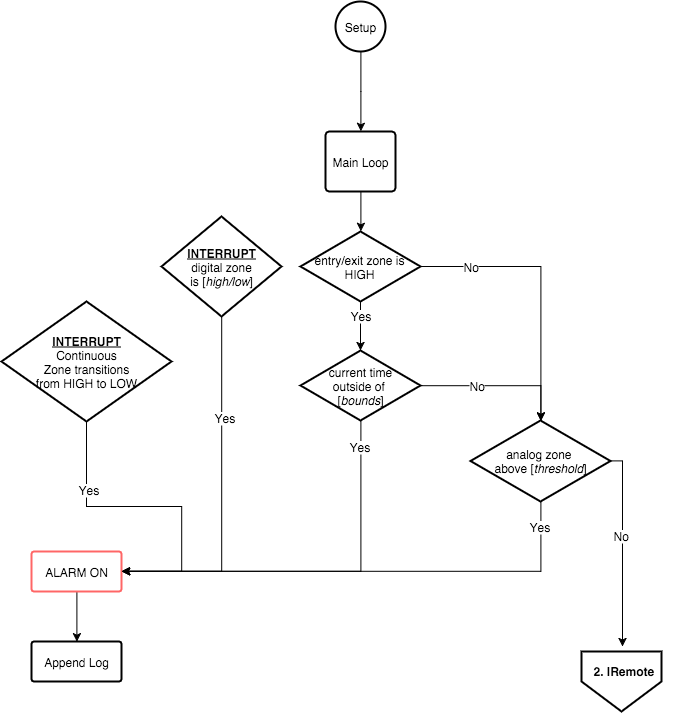
\includegraphics[width=20.5cm]{ControlFlow/1_ControlFlowDiagram.png}}
\newpage
\makebox[\textwidth]{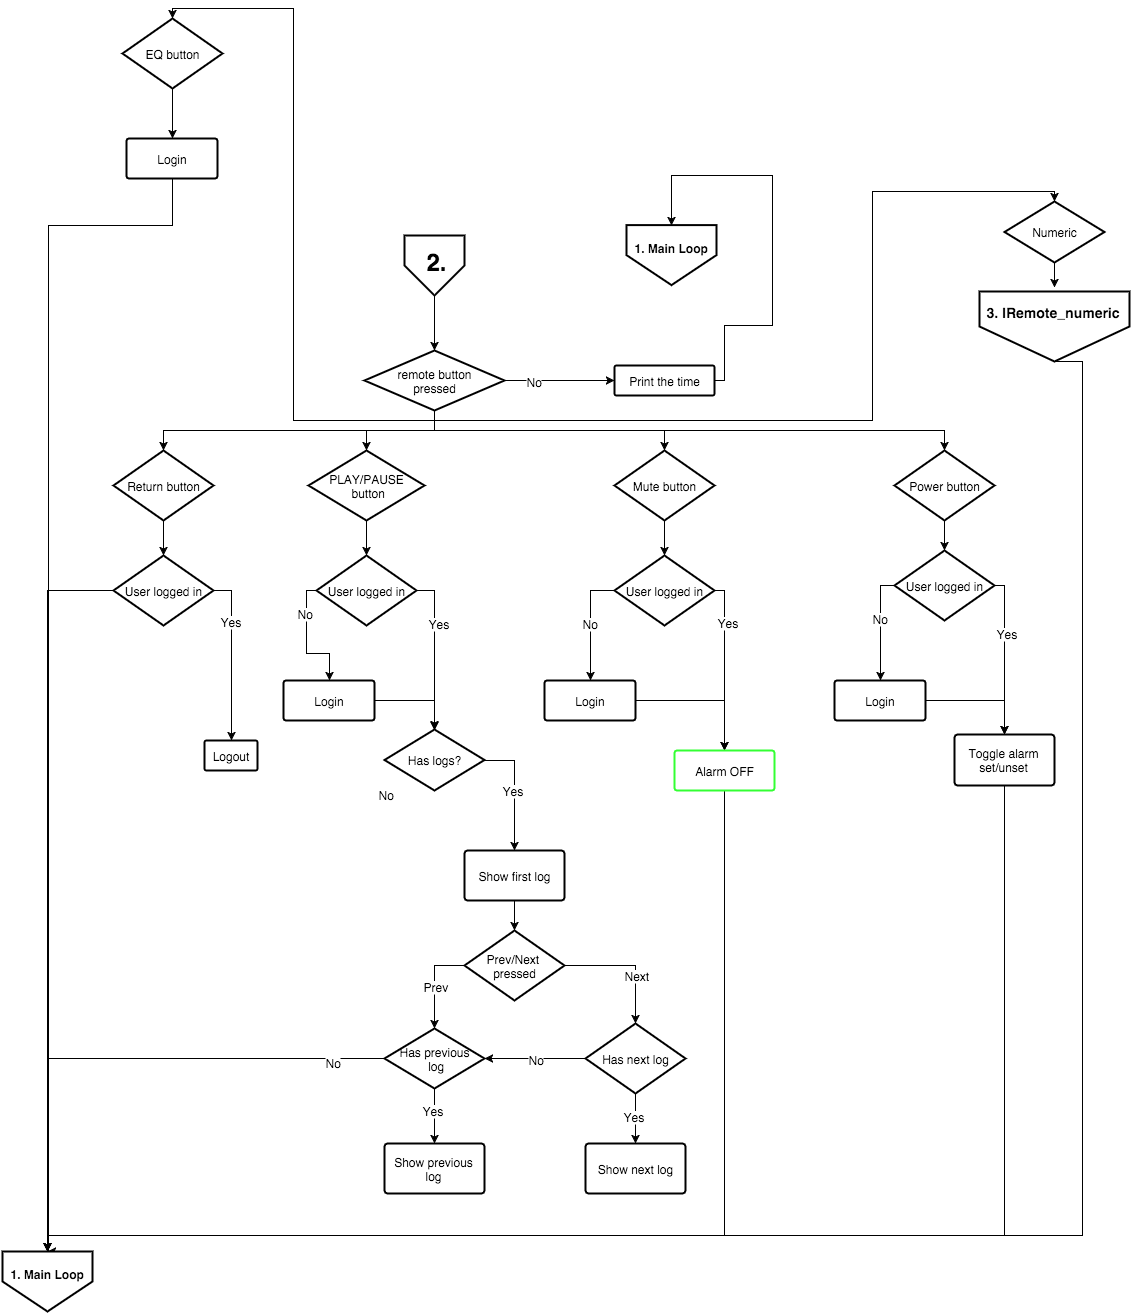
\includegraphics[width=20.5cm]{ControlFlow/2_IRemote.png}}
\makebox[\textwidth]{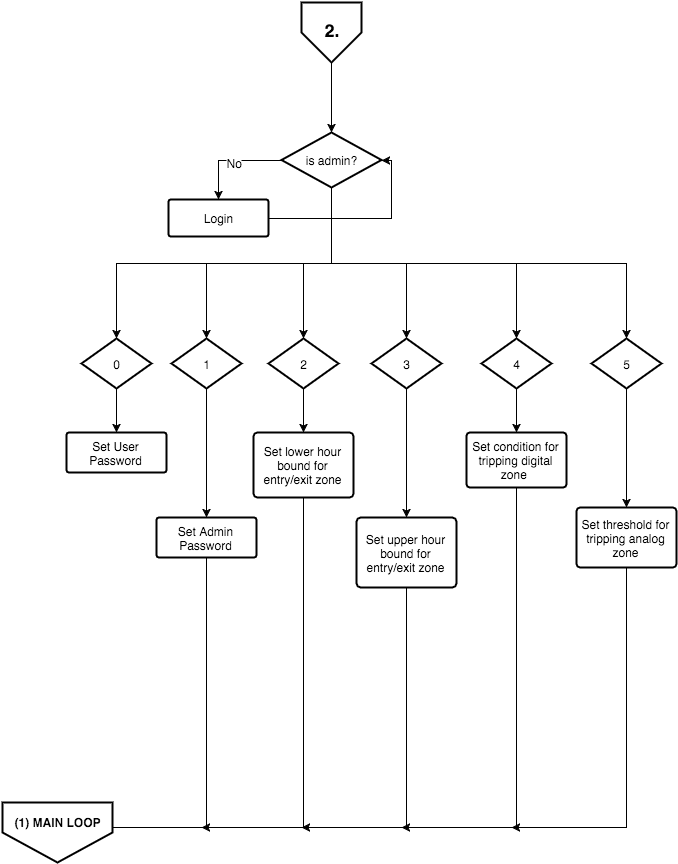
\includegraphics[width=20.5cm]{ControlFlow/3_IRemote_numeric.png}}

\subsection{Circuit Diagram}
\makebox[\textwidth]{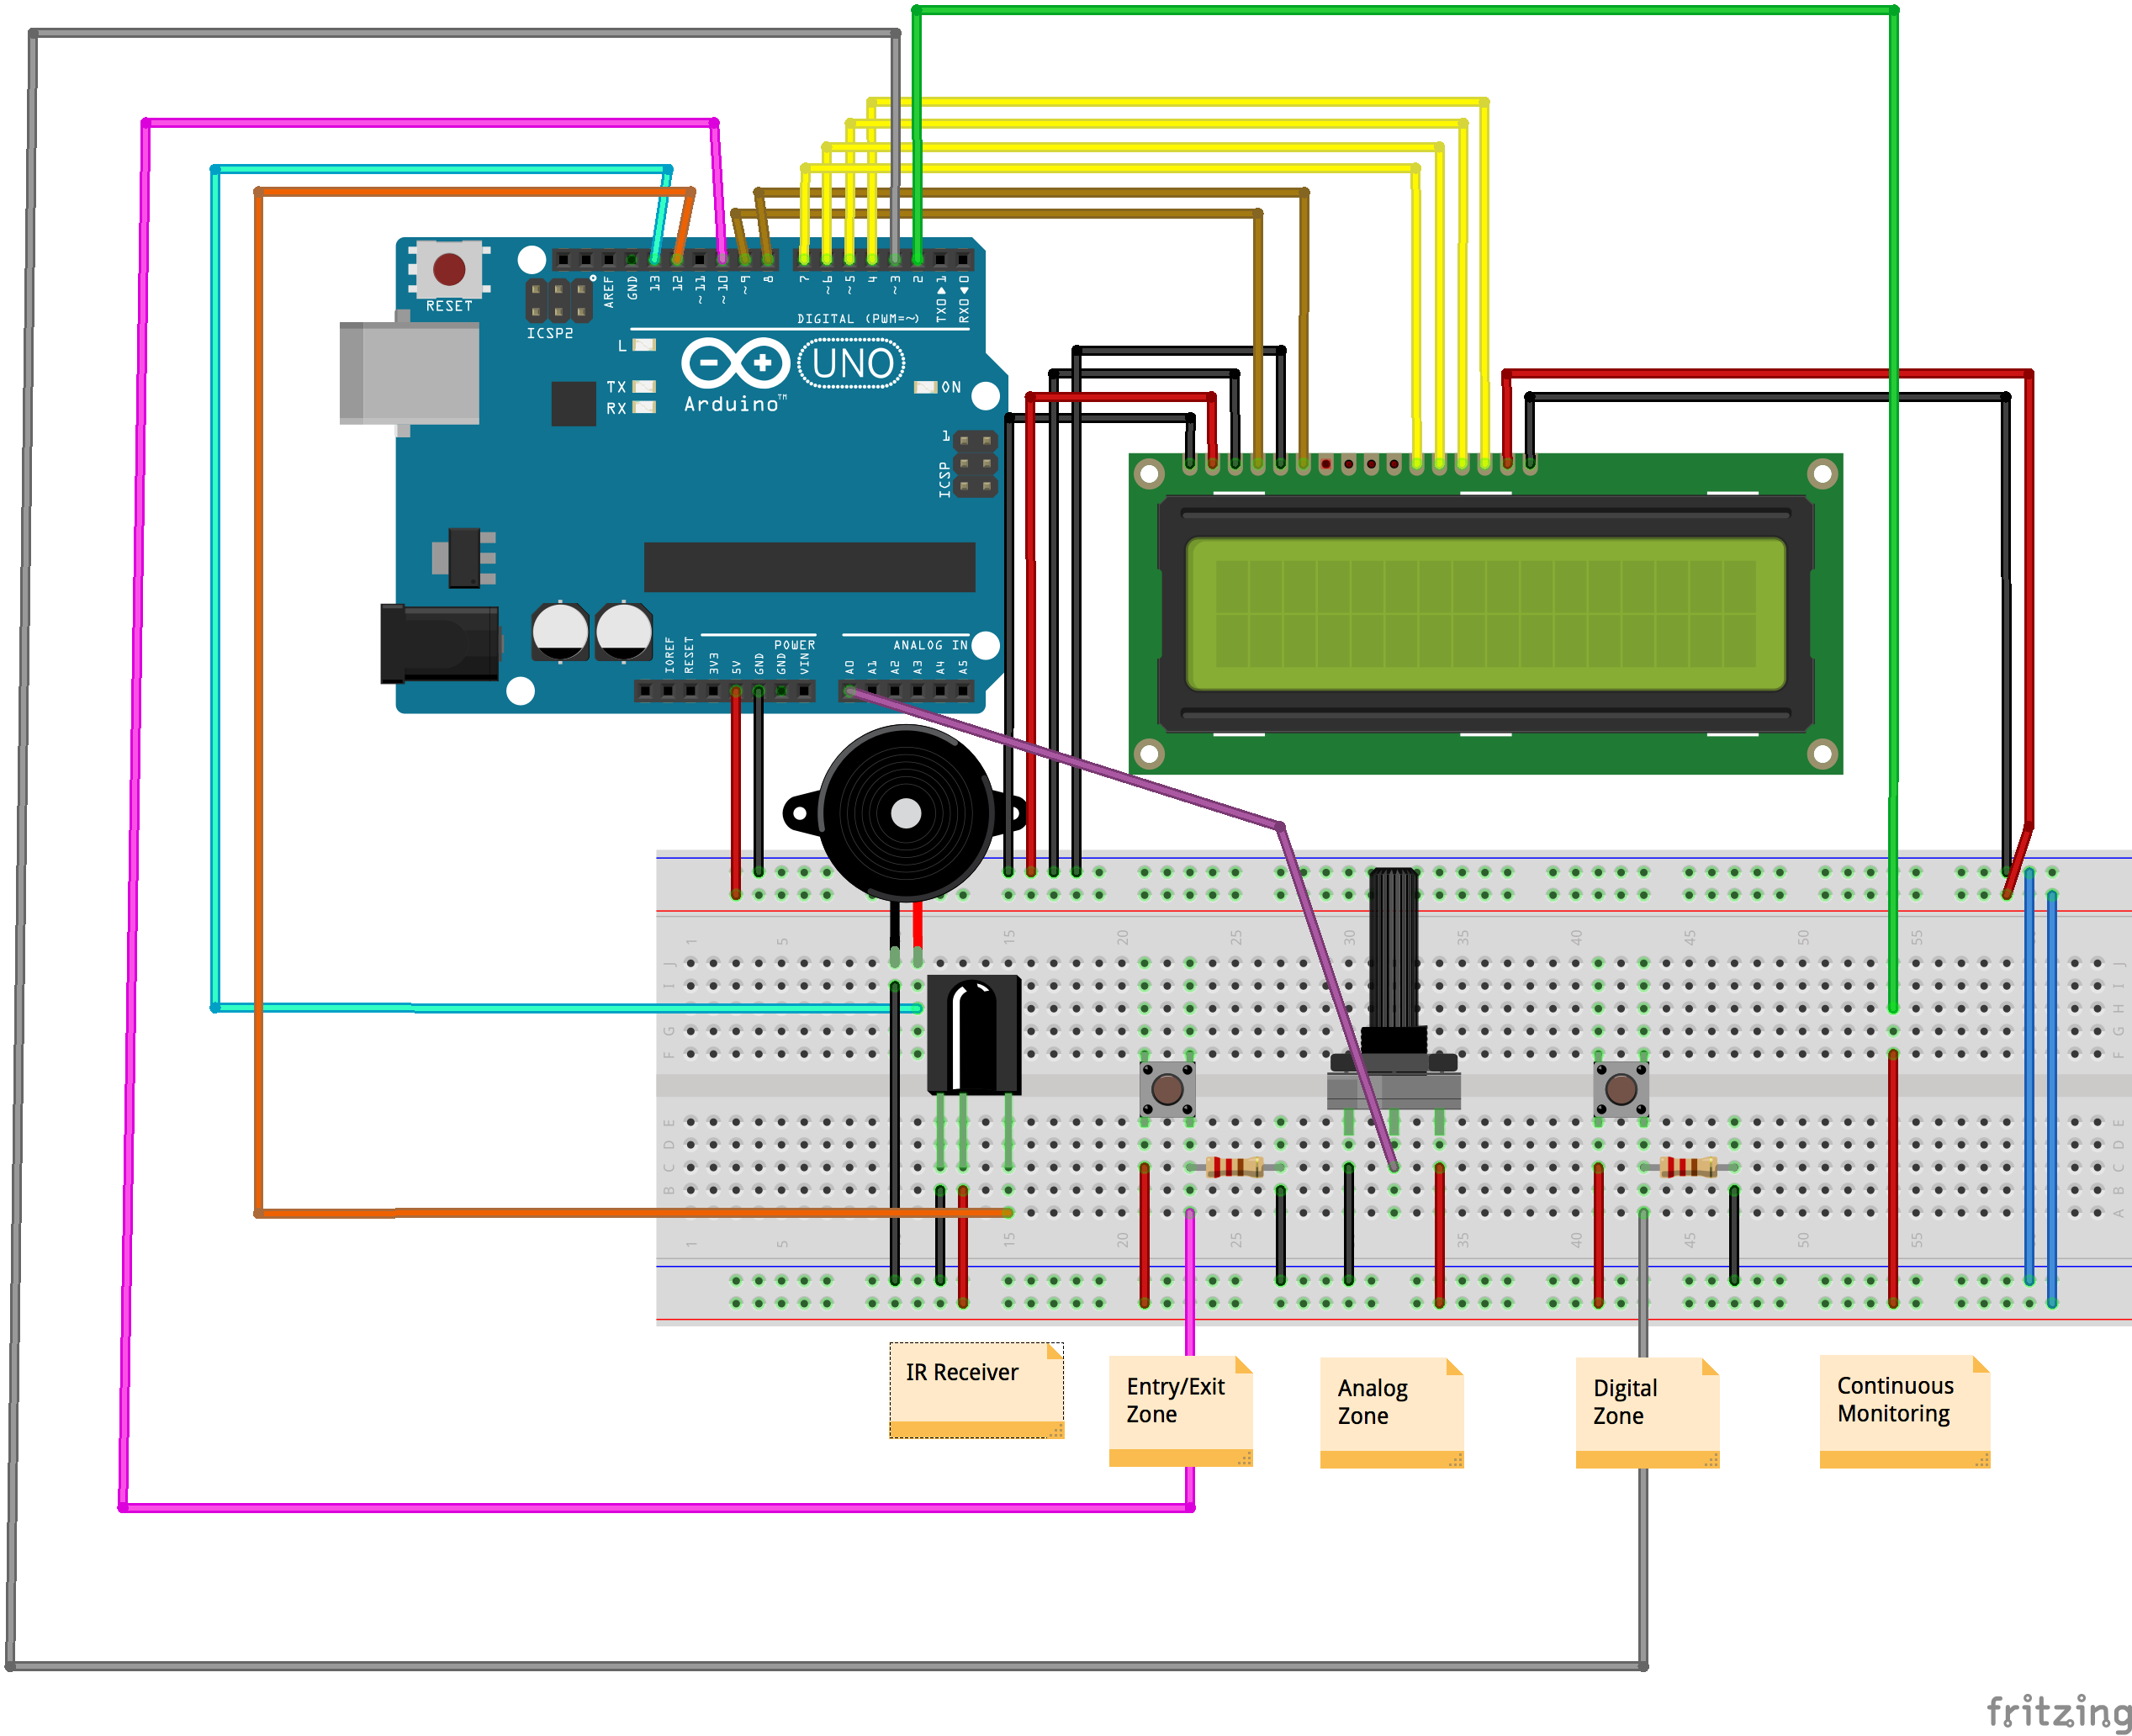
\includegraphics[width=20.5cm]{Circuit/CircuitDiagram_bb.png}}

\subsection{Coding decisions}

\subsubsection{Global Variables}
We decided to have five global variables:

\begin{lstlisting}
// initialize the library with the numbers of the interface pins
LiquidCrystal lcd(9, 8, 7, 6, 5, 4);

// Used to check if current user is an admin
unsigned short is_admin = 0;

// 0 is disabled ; 1 is enabled
unsigned short alarm_set = 0;

// 0 alarm is idle ; 1 alarm is ringing
// Volatile because needed in interrupts
volatile unsigned short alarm_active = 0;

// 0 not logged in ; 1 logged in 
unsigned short is_user_logged_in = 0;
\end{lstlisting}

All of these variables are used extensively within other functions for manipulation of the components overall, which is the reason they've been globalised.

\subsubsection{Debouncing IR}

At many points in our code, we add a delay after receiving a numeric signal from the IR Remote in order to prevent extraneous zeroes corrupting the intended number.

\subsubsection{Default Settings on First Time}

When the microcontroller is first setup, we should populate the EEPROM with default settings. Depending on the use of the microcontroller before this program was uploaded, the EEPROM may have old values still stored in its memory so we chose a sentinel value - a 3-byte char - to tell whether the defaults had been set or not. 

\subsubsection{Digital and Continuous Zones are interrupts}

We chose to make the digital and continuous zones as interrupts to simplify the code and make the alarm more responsive.

The continuous zone interrupts on a falling signal only so when the signal goes from HIGH to LOW, the alarm is set off as the wire connection has been broken.

The digital zone interrupts whenever the signal changes and then checks it against the user-defined condition. If the condition is met, the alarm goes off.

\begin{lstlisting}
attachInterrupt( digitalPinToInterrupt(DIGITAL_ZONE_PIN), digitalZoneTrip, CHANGE  );
attachInterrupt( digitalPinToInterrupt(CONTINUOUS_ZONE_PIN), contZoneTrip, FALLING );
\end{lstlisting}

\subsubsection{Check For Admin}
\begin{lstlisting}
if( is_admin || ( loginMode( ) && is_admin ) )
\end{lstlisting}

Whenever we needed an admin login to change settings, etc., we used the fact that C lazy-evaluates to our advantage. If the admin was already logged in, he passed into the statement immediately but if we had to make them login, we used the fact that C evaluates logic conditions from left to right. So first the admin would login and if they were successful, then the \inlinecode{is_admin} flag would be set and we could let them in.

\subsubsection{Logs Loop}

\begin{lstlisting}
int memory_address = LOG_MEMORY_START + (( LOG_MEMORY_START + (LOG_LENGTH * number_of_breaches) ) % 500);
\end{lstlisting}

When storing a log, if we've reached the maximum space (in this case it's 500 bytes to be safe), we loop around and continue writing logs at the beginning of the memory.

\subsubsection{Increased Extensibility for Logging}
\begin{lstlisting}
EEPROM.put( memory_address, time_of_breach );
memory_address += sizeof(time_of_breach);
EEPROM.put( memory_address, (short) zone );
\end{lstlisting}

By using sizeof, we don't have to store a constant with the size of the time variable so we could easily increase the \inlinecode{LOG_LENGTH} constant, add the size of the \inlinecode{zone} variable to the memory address and then write a new variable/value as part of the log.


\section{Evaluation}
\subsection{How successful was it?}
The burglar alarm works as expected but the continuous zone was hard to conceptually understand. We chose a more low-tech, physical approach which achieved the same outcome but was probably not what was sought.

The EEPROM works exceptionally well and leaves a lot of room for additional settings if needed later. 

The analog zone works exactly as expected with the potentiometer as an example.

Attaching the digital and continuous zone to interrupts simplified our code and gives a much more instantaneous response to actions.

The entry/exit zone also works quite nicely despite requiring us to poll for it in the loop. The countdown upon entering the house also works a lot better than expected although the count stops while trying to login so you could theoretically enter login multiple times to keep the alarm occupied while you disabled it.

\subsection{Any improvements?}
We spent a portion of the project misunderstanding that both short and int occupy the same number of bytes, I would probably stick solely to using int data types now knowing this.

Now understanding the role of the continuous monitoring zone more closely, I would probably look at embedding software and circuity in other zones to ensure they're operating as expected instead of our proposed approach.

I would probably create an interrupt for timing so that we could continue to count time as someone's trying to login to the entry/exit zone. I would also set the alarm off on a failed login to avoid a brute force attack.

Logs loop but start muddying the order. We could probably fix this by also storing a sequence number and navigating through them that way.

Because so many of our settings (EG: Digital condition and the upper/lower bound hours) only needed less than 1 byte for storage but took up 2 bytes as ints, we could probably use a single int to store two settings.
\section{Appendices}
\begin{lstlisting}

\end{lstlisting}


\subsection{User manual}
\makebox[\textwidth]{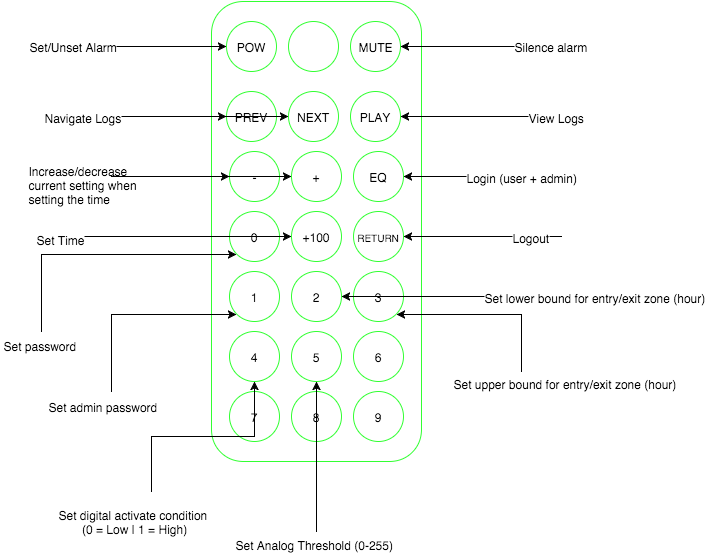
\includegraphics[width=20.5cm]{Manual/IR_Remote_Diagram.png}}

\subsubsection{How do I silence the alarm?}
When the alarm is active/sounding, you can silence it using the "Mute" button in the top-right corner of the remote. You will be asked to login (enter your passcode) to deactivate it unless you have recently logged in (\textit{and have not SET the alarm}).

\subsubsection{When will the alarm activate?}
\begin{itemize}
    \item \textbf{Analog Zone:} When the desired threshold is exceeded, the alarm will activate.
    \item \textbf{Digital Zone:} When the chosen condition is met (HIGH/LOW), the alarm will activate.
    \item \textbf{Entry/Exit Zone:} When you enter the house, you will be given 20 seconds to login and deactivate the alarm. The alarm \textbf{will not} activate if you enter your home between the two hours you've selected in the options.
    \item \textbf{Continuous Zone:} When the seal of the box is broken, the two wires connected to the lid of the container will separate and the alarm will sound. This is an anti-tampering measure as the user should never be altering the direct wiring of the alarm after setup.
\end{itemize}

Whenever a zone is tripped, a log of the zone, the date and the time is written to memory for you to browse later. To view logs, hit the play/pause button and use the prev and next buttons to navigate through them.


\subsection{Project plan}
\begin{enumerate}
    \item Map out the EEPROM memory
    \item Assign functions to IR Remote buttons
    \item Map all necessary pins to relevant components
    \item Declare constants at the top of the code
    \item Begin outlining the code
    \item Assemble the hardware for testing
    \item Test, re-iterate
    \item Finalise the code and hardware and test again
\end{enumerate}

Throughout the project, we used Github to organise our code and traded the arduino back and forth as we tackled separate hardware problems and ideas.

\subsubsection{EEPROM Mapping}
\begin{lstlisting}
/**
 * EEPROM Mapping
 * --------------
 * 0 - 1 : password (unsigned int)
 * 2 - 3 : admin password (unsigned int)
 * 4 - 5 : number of breaches (unsigned short)
 * 6 - 8 : first-time settings ("set" or anything else)
 *
 *  Entry/Exit (Zone 0)
 *    15     : lower-bound hour (unsigned short)
 *    16     : upper-bound hour (unsigned short)
 *
 *  Digital (Zone 1)
 *    20    : trip condition (unsigned short)
 *    
 *  Analog  (Zone 2)
 *    30 - 32 : threshold (unsigned int)
 *
 * 100 - 511 : Logging
 *   Bit Mapping (6 bytes each):
 *   0 - 3 : time (unsigned long int)
 *   4 - 5 : zone (unsigned short)
 *   
 */
\end{lstlisting}

\subsubsection{IR Button Mapping}
\begin{lstlisting}
/**
 * IR Remote Layout
 * ----------------
 *
 * EQ : Enter password (4-Digit Pin)
 * Return : Return to standard menu
 * Play/Pause : Navigate Log
 *   Next     : Next log
 *   Prev     : Previous log
 * Mute       : Turn off alarm
 * Power      : Set/unset the alarm
 * 0  : Set user password
 * 1  : Set admin password
 * 2  : Set lower bound hour for entry/exit zone
 * 3  : Set upper bound hour for entry/exit zone
 * 4  : Set digital activate condition
 * 5  : Set analog threshold
 */
\end{lstlisting}

\subsubsection{Pin Mapping}
\begin{lstlisting}
/**
 * Digital
 * -------
 * 
 * 2 (interrupt) : Continuous Zone 
 * 3 (interrupt) : Digital Zone
 * 4 : LCD Screen 
 * 5 : LCD Screen
 * 6 : LCD Screen
 * 7 : LCD Screen
 * 8 : LCD Screen
 * 9 : LCD Screen
 * 10: Entry/Exit Zone
 * 12: IR Sensor
 * 13: ALARM
 * 
 * Analog
 * ------
 * 0 : Analog Zone 1
 */
\end{lstlisting}

\section{Code}

\begin{lstlisting}
#include <EEPROM.h>
#include <Time.h>  
#include <IRremote.h>
#include <LiquidCrystal.h>

/**
 * @author Colm Cahalane
 * @author Evan Smith <113300626>
 *
 * Build a burglar alarm --- The task for the project 
 * was to build a device, using an arduino, that could 
 * monitor several different types of zones, log alarm
 * trips and allow for user and admin interaction via 
 * an LCD. When an alarm condition is met, a buzzer 
 * or LED will go off indicating as such.
 * 
 * Pins
 * ====
 * 
 * Digital
 * -------
 * 
 * 2 (interrupt) : Continuous Zone 
 * 3 (interrupt) : Digital Zone
 * 4 : LCD Screen 
 * 5 : LCD Screen
 * 6 : LCD Screen
 * 7 : LCD Screen
 * 8 : LCD Screen
 * 9 : LCD Screen
 * 10: Entry/Exit Zone
 * 12: IR Sensor
 * 13: ALARM
 * 
 * Analog
 * ------
 * 0 : Analog Zone 1
 *
 * IR Remote Layout
 * ----------------
 *
 * EQ : Enter password (4-Digit Pin)
 * Return : Return to standard menu
 * Play/Pause : Navigate Log
 *   Next     : Next log
 *   Prev     : Previous log
 * Mute       : Turn off alarm
 * Power      : Set/unset the alarm
 * 0  : Set user password
 * 1  : Set admin password
 * 2  : Set lower bound hour for entry/exit zone
 * 3  : Set upper bound hour for entry/exit zone
 * 4  : Set digital activate condition
 * 5  : Set analog threshold
 *
 * EEPROM Mapping
 * --------------
 * 0 - 1 : password (unsigned int)
 * 2 - 3 : admin password (unsigned int)
 * 4 - 5 : number of breaches (unsigned short)
 * 6 - 8 : first-time settings ("set" or anything else)
 *
 *  Entry/Exit (Zone 0)
 *    15     : lower-bound hour (unsigned short)
 *    16     : upper-bound hour (unsigned short)
 *
 *  Digital (Zone 1)
 *    20    : trip condition (unsigned short)
 *    
 *  Analog  (Zone 2)
 *    30 - 32 : threshold (unsigned int)
 *
 * 100 - 511 : Logging
 *   Bit Mapping (6 bytes each):
 *   0 - 3 : time (unsigned long int)
 *   4 - 5 : zone (unsigned short)
 *   
 *   
 */

#define PASSWORD              0     // 4 digit pin
#define ADMIN_PASSWORD        2     // 4 digit pin
#define NUMBER_OF_BREACHES    4
#define FIRST_TIME_SET        6

// ~~~~~ ENTRY / EXIT ZONE ~~~~~
#define ENTRY_EXIT_ZONE       0
#define ENTRY_EXIT_PIN        10
#define LOWER_TIME_BOUND      15     // Hour (2 digits max)
#define UPPER_TIME_BOUND      16     // Hour (2 digits max)

// ~~~~~~~ DIGITAL ZONE ~~~~~~~~
#define DIGITAL_ZONE          1
#define DIGITAL_CONDITION     20    // HIGH (1) or LOW (0)
#define DIGITAL_ZONE_PIN      3

 // ~~~~~~~ ANALOG ZONE ~~~~~~~~
#define ANALOG_ZONE           2
#define ANALOG_THRESHOLD      30    // short between 0 - 255
#define ANALOG_ZONE_PIN       0


 // ~~~ CONTINUOUS MON ZONE ~~~~
#define CONTINUOUS_ZONE       3
#define CONTINUOUS_ZONE_PIN   2

 // ~~~~~ TIME SETTING MODE ~~~~
#define HOUR 0
#define MINUTE 1
#define DAY 2
#define MONTH 3
#define YEAR 4

// ~~~~~~~~~ LOGS ~~~~~~~~~~~~~~
#define LOG_MEMORY_START  100
#define LOG_LENGTH        6

// ~~~~~~~~~~ IR ~~~~~~~~~~~~~~~
#define IR_RECV_PIN   12
IRrecv irrecv(IR_RECV_PIN);
decode_results results;

#define ALARM_PIN     13

// initialize the library with the numbers of the interface pins
LiquidCrystal lcd(9, 8, 7, 6, 5, 4);

// Used to check if current user is an admin
unsigned short is_admin = 0;

// 0 is disabled ; 1 is enabled
unsigned short alarm_set = 0;

// 0 alarm is idle ; 1 alarm is ringing
volatile unsigned short alarm_active = 0;

// 0 not logged in ; 1 logged in 
unsigned short is_user_logged_in = 0;

/**
 * Prints the current time to the LCD
 */
void printTime(){
  lcd.setCursor(0, 0);
  convertUnixToReadable(now());
}

/**
 * Pads and prints an integer with 0s
 * @param val Integer to pad
 */
void printWithLeadingZero(int val){
  if(val < 10){
    lcd.print('0');
  }
  lcd.print(val);
}

/**
 * Set the time
 */
void changeTime(){
    TimeElements t;
    time_t newTime;
    breakTime(now(), t);
    
    int settingsMode = 0;
    short exitLoop = 0;

    while( !exitLoop ){
      newTime = makeTime(t);
  
      lcd.clear();
      lcd.setCursor(0,0);

      lcd.print( hour(newTime) );
      lcd.print(':');
      printWithLeadingZero( minute(newTime) );

      lcd.print(' ');

      printWithLeadingZero( day(newTime) );
      lcd.print('/');
      printWithLeadingZero( month(newTime) );
      lcd.print('/');
      lcd.print( year(newTime) );

      lcd.setCursor(0,1);
      
      if(settingsMode == HOUR){
        lcd.print("Setting HOUR");
      } else if(settingsMode == MINUTE){
        lcd.print("Setting MINUTE");
      } else if(settingsMode == DAY){
        lcd.print("Setting DAY");
      } else if(settingsMode == MONTH){
        lcd.print("Setting MONTH");
      } else if(settingsMode == YEAR){
        lcd.print("Setting YEAR");
      }

      irrecv.resume();
      while( !irrecv.decode(&results) ) { /* Wait for input! */ }
      switch(results.value){
                            // +4 should be -1, but here we avoid nevative modulo
        case 0xFF22DD: /* PREV */ settingsMode = (settingsMode+4)%5;       break;
        case 0xFF02FD: /* NEXT */ settingsMode = (settingsMode+1)%5;       break;
        case 0xFFE01F: /*  -  */
            if(settingsMode == HOUR){
              t.Hour--;
            } else if(settingsMode == MINUTE){
              t.Minute--;
            } else if(settingsMode == DAY){
              t.Day--;
            } else if(settingsMode == MONTH){
              t.Month--;
            } else if(settingsMode == YEAR){
              t.Year--;
            }
           break;
        case 0xFFA857: /*  +  */
            if(settingsMode == HOUR){
              t.Hour++;
            } else if(settingsMode == MINUTE){
              t.Minute++;
            } else if(settingsMode == DAY){
              t.Day++;
            } else if(settingsMode == MONTH){
              t.Month++;
            } else if(settingsMode == YEAR){
              t.Year++;
            }
           break;
        case 0xFFB04F: /* RET */ exitLoop = 1; lcd.clear(); break;
      }
    }

    setTime(newTime);
}

int getDigitFromIR(){
  while( 1 ){
    irrecv.resume();
    while( !irrecv.decode(&results) ) { /* Wait for input! */ }
    switch(results.value)
    {
      case 0xFF6897: return 0;
      case 0xFF30CF: return 1;
      case 0xFF18E7: return 2;
      case 0xFF7A85: return 3;
      case 0xFF10EF: return 4;
      case 0xFF38C7: return 5;
      case 0xFF5AA5: return 6;
      case 0xFF42BD: return 7;
      case 0xFF4AB5: return 8;
      case 0xFF52AD: return 9;
      default:       break; // Other button press or undefined; reloop
    }
  }
}

/**
 * Attempt to log in a user, prompting
 *   them for a user or admin password
 * @return 1 if user logged in ; 0 otherwise
 */
int loginMode() {
  lcd.clear();
  lcd.print( "Login Mode");
  if( !is_user_logged_in || !is_admin ){
    // if admin is already logged in, bypass login

    lcd.clear();
    if( is_user_logged_in && !is_admin ){
      lcd.print( "Enter admin pin");
    } else {
      lcd.print( "4 Digit Pin");
    }
    delay(50);
    
    int pin_entered = 0;
    unsigned int password, admin_password;
    EEPROM.get( PASSWORD, password );
    EEPROM.get( ADMIN_PASSWORD, admin_password );

    lcd.setCursor(0, 1);
    for(int i = 0; i < 4; i++){
      int received_value = getDigitFromIR();      
      pin_entered *= 10;
      pin_entered += received_value;
      lcd.print('*');

      // Minor delay to prevent debouncing "0"s
      delay(50);
      irrecv.resume();
    }


    lcd.setCursor(0,1);
    if( !is_user_logged_in && pin_entered == password ){
      is_user_logged_in = 1;
      lcd.print( "LOGGED IN" );
    } else if( pin_entered == admin_password ){
      is_admin = 1;
      is_user_logged_in = 1;
      lcd.print( "LOGGED IN" );
    } else{
      lcd.print( "FAILED LOGIN" );
    }
    delay(1500);
  } else{
    lcd.print("You are admin");
  }
  lcd.clear();
  
  return is_user_logged_in;
}

/**
 * Append log to memory
 * @param time_of_breach Unix timestamp of current time
 * @param zone           Zone number that was breached
 */
void appendLog( unsigned long int time_of_breach, unsigned short zone ){

  unsigned short number_of_breaches;
  EEPROM.get( NUMBER_OF_BREACHES, number_of_breaches );

  // Increase the number of breaches
  number_of_breaches++;
  EEPROM.put( NUMBER_OF_BREACHES, number_of_breaches );

  int memory_address = LOG_MEMORY_START + (( LOG_MEMORY_START + (LOG_LENGTH * number_of_breaches) ) % 500);

  // Write our log to EEPROM
  EEPROM.put( memory_address, time_of_breach );
  memory_address += sizeof(time_of_breach);
  EEPROM.put( memory_address, (short) zone );
}

/**
 * Allows user to navigate the stored log
 * @param current_log The current log to be printed
 */
void printLog( short current_log ){
  unsigned short number_of_breaches;
  EEPROM.get( NUMBER_OF_BREACHES, number_of_breaches );

  if( current_log <= number_of_breaches && current_log != 0){
    // If we have a log to show 
    int memory_address = LOG_MEMORY_START + (( LOG_MEMORY_START + (LOG_LENGTH * current_log) ) % 500);
    
    unsigned long int time_of_breach;
    unsigned short zone;

    // Get log info
    EEPROM.get( memory_address, time_of_breach );
    memory_address += sizeof(time_of_breach);
    EEPROM.get( memory_address, zone );
    
    lcd.clear();
    switch(zone){
      case DIGITAL_ZONE:
          lcd.print( "DIGITAL ZONE");
        break;
      case ANALOG_ZONE:
          lcd.print("ANALOG ZONE");
        break;
      case CONTINUOUS_ZONE:
          lcd.print( "CONTINUOUS ZONE");
        break;
      case ENTRY_EXIT_ZONE:
          lcd.print("ENTRY/EXIT ZONE");
        break;
      default:
          lcd.print( "UNKNOWN ZONE" );
        break;
    }
    lcd.setCursor(0,1);
    convertUnixToReadable( time_of_breach );

    irrecv.resume();
    while( !irrecv.decode(&results) ) { /* Wait for input! */ }
    switch(results.value)
    {
      case 0xFF22DD: printLog( current_log - 1 );    break;
      case 0xFF02FD: printLog( current_log + 1 );    break;
      case 0xFFB04F: lcd.clear(); /* If return, just let it go */ break;
      default: printLog(current_log); // Other button press or undefined
    }
    irrecv.resume();
  } else{
    lcd.clear();
    lcd.print("NO LOGS");
    delay( 1000 );

    if( current_log > 0 )
      // If current log isn't 0, send them back a log
      printLog( current_log - 1 );
  }
}

/**
 * Prints out unix time in a human-readable format
 * @param  input_time Unix time input
 */
void convertUnixToReadable( unsigned long int input_time ){
  TimeElements full_time;
  breakTime( input_time, full_time );

  printWithLeadingZero(full_time.Hour);
  lcd.print( ":" );
  printWithLeadingZero(full_time.Minute); 
  lcd.print( " " );
  printWithLeadingZero( full_time.Day );
  lcd.print("/");
  printWithLeadingZero( full_time.Month );
  lcd.print("/");
  lcd.print( full_time.Year + 1970 );
}

/**
 * Exit admin mode
 */
void exitAdmin( ){
  is_admin = 0;
  logout( );
}

/**
 * Remove logged in status
 */
void logout( ){
  is_user_logged_in = 0;
  lcd.clear();
  lcd.print("Logged out");
  delay(700);
}

/**
 * Change whether the alarm can be active or not
 */
void toggleAlarmSet( ){
  if( !alarm_active ){
    lcd.clear();
    // We set the alarm at the end of the function to
    // avoid interrupts triggering the alarm
    unsigned short temp_alarm = !alarm_set;
    
    if( temp_alarm ){
      logout( );
      for (int i = 9; i < 10 && i >= 0; i--){
        lcd.clear();
        lcd.print(i);
        delay(1000);
      }
      lcd.clear();
      lcd.print( "ALARM SET" );
      delay(800);
    } else{
      lcd.print( "ALARM UNSET" );
      delay(800);
    }

    alarm_set = temp_alarm;
  }
}

/**
 * Change whether alarm is ringing or not
 */
void toggleAlarm( ){
  alarm_active = !alarm_active;

  lcd.clear();
  lcd.setCursor(0,1);
  if( alarm_set ){
    if( alarm_active ){
      lcd.print( "ALARM ACTIVE     " );
      digitalWrite( ALARM_PIN, HIGH );
    } else {
      lcd.print( "ALARM DEACTIVATED" );
      digitalWrite( ALARM_PIN, LOW );
      delay(1500);
      lcd.clear();
    }
  }
}


/**
 * Trip the digital zone if conditions are met
 */
void digitalZoneTrip( ){
  volatile unsigned short trip_condition;
  EEPROM.get( DIGITAL_CONDITION, trip_condition );

  if( trip_condition ){
    if( digitalRead( DIGITAL_ZONE_PIN ) == HIGH && !alarm_active && alarm_set ){
      toggleAlarm( );
      appendLog( now(), DIGITAL_ZONE );
    }
  } else {
    if( digitalRead( DIGITAL_ZONE_PIN ) == LOW && !alarm_active && alarm_set ){
      toggleAlarm( );
      appendLog( now(), DIGITAL_ZONE );
    }
  }
}

/**
 * Trip the continuous zone
 */
void contZoneTrip( ){
  toggleAlarm( );
  appendLog( now(), CONTINUOUS_ZONE );
}

/**
 * Trip the analog zone if higher than threshold
 */
void analogZoneTrip( ){
  unsigned int threshold;
  EEPROM.get( ANALOG_THRESHOLD, threshold );

  if( analogRead( ANALOG_ZONE_PIN ) > threshold && !alarm_active && alarm_set ){
    toggleAlarm( );
    appendLog( now(), ANALOG_ZONE );
    delay(200);
  }
}

/**
 * Allows users to set permanent option 
 *   values (stored in EEPROM)
 * @param option Option number from IR Remote
 */
void setOption( short option ){
  unsigned int address;
  unsigned short digits;
  switch( option ){
    case 0:
        lcd.print("PASSWORD");
        address = PASSWORD;
        digits = 4;
      break;
    case 1:
        lcd.print("ADMIN_PASSWORD");
        address = ADMIN_PASSWORD;
        digits = 4;
      break;
    case 2:
        lcd.print("LOWER TIME (Hour)");
        address = LOWER_TIME_BOUND;
        digits = 2;
      break;
    case 3:
        lcd.print("UPPER TIME (Hour)");
        address = UPPER_TIME_BOUND;
        digits = 2;
      break;
    case 4:
        lcd.print("DIGITAL COND 0/1");
        address = DIGITAL_CONDITION;
        digits = 1;
      break;
    case 5:
        lcd.print("ANALOG THRESH 1-255");
        address = ANALOG_THRESHOLD;
        digits = 3;
      break;
    default:
        return;
      break;
  }

  if( digits > 2 ){
    // If there are more than 2 digits, we'll need an int
    unsigned int final_value = 0;
    lcd.setCursor(0,1);
    for(int i = 0; i < digits; i++){
      int received_value = getDigitFromIR();
        final_value *= 10;
        final_value += received_value;
        lcd.print(received_value);
        // Minor delay to prevent debouncing "0"s
        delay(50);
        irrecv.resume();
    }
    EEPROM.put( address, final_value );
  } else {
    // If there are less than 2 digits, we can use a short
    unsigned short final_value = 0;
    lcd.setCursor(0,1);
    for(int i = 0; i < digits; i++){
      int received_value = getDigitFromIR();
        final_value *= 10;
        final_value += received_value;
        lcd.print(received_value);
        // Minor delay to prevent debouncing "0"s
        delay(50);
        irrecv.resume();
    }
    EEPROM.put( address, final_value );
  }
}

/**
 * Places default values in memory if it's the 
 * first time
 */
void defaults(){
  unsigned int password = 1234, 
               admin_password = 5678, 
               analog_threshold = 100;

  unsigned short number_breaches = 0,
                 lower_bound_hour = 20,
                 upper_bound_hour = 22,
                 digital_trip_condition = 1;

  char first_time[] = "SET";
  EEPROM.put( FIRST_TIME_SET, first_time );
  EEPROM.put( PASSWORD, password );
  EEPROM.put( ADMIN_PASSWORD, admin_password );
  EEPROM.put( ANALOG_THRESHOLD, analog_threshold );

  EEPROM.put( NUMBER_OF_BREACHES, number_breaches );
  EEPROM.put( LOWER_TIME_BOUND, lower_bound_hour );
  EEPROM.put( UPPER_TIME_BOUND, upper_bound_hour );
  EEPROM.put( DIGITAL_CONDITION, digital_trip_condition );
}

/**
 * Check if settings exist
 * @return 0 if not first time; 1 if first time
 */
int settingsSet( ){
  char first_time[3];

  EEPROM.get( FIRST_TIME_SET, first_time );

  return !(first_time == "SET");
}

void setup() {
  Serial.begin(9600);

  pinMode(ALARM_PIN, OUTPUT);
  pinMode(CONTINUOUS_ZONE_PIN, INPUT);
  pinMode(DIGITAL_ZONE_PIN, INPUT);
  pinMode(ENTRY_EXIT_PIN, INPUT);

  digitalWrite( ALARM_PIN, LOW );
  digitalWrite( CONTINUOUS_ZONE_PIN, LOW );
  digitalWrite( DIGITAL_ZONE_PIN, LOW );

  attachInterrupt( digitalPinToInterrupt(DIGITAL_ZONE_PIN), digitalZoneTrip, CHANGE  );
  attachInterrupt( digitalPinToInterrupt(CONTINUOUS_ZONE_PIN), contZoneTrip, FALLING );

  int first_time = settingsSet( );

  if( first_time ){
    defaults();
  }

  alarm_set = 0;
  
  setTime( 1447854337 );
      
  irrecv.enableIRIn(); 

  lcd.begin(16, 2);
}

void loop() {

  /**
   * Trip the Entry/Exit zone as necessary
   */
  if( digitalRead(ENTRY_EXIT_PIN) == HIGH ){
    unsigned short lower, upper, currentHour;
    EEPROM.get( LOWER_TIME_BOUND, lower );
    EEPROM.get( UPPER_TIME_BOUND, upper );
    currentHour = hour();

    lcd.clear();
    lcd.print("Plz login (EQ)");
    long start_time = millis();
    lcd.setCursor(0,1);
    while( (millis() - start_time) < 20000 ){
       
      irrecv.resume();
      delay(300);
      if(irrecv.decode(&results)){  
        if( results.value == 0xFF906F ){
          if( !is_user_logged_in ){
           loginMode( );
          }
          lcd.clear();
          lcd.print("Crisis averted");
          delay(800);
          break;
        }
      }
      lcd.clear();
      lcd.print("Plz login (EQ)");
      lcd.setCursor(0,1);
      lcd.print( 20 - ((millis() - start_time) / 1000) );
    }
    irrecv.resume(); 

    if( !alarm_active && alarm_set && !( currentHour <= lower && currentHour >= upper) ){
      // If current hour is not between the upper and lower bound
      // then activate the alarm
      toggleAlarm( );
      appendLog( now(), ENTRY_EXIT_ZONE );
      delay( 200 );
    }
  }
  
  analogZoneTrip( );

  if( irrecv.decode(&results) ) {
    switch(results.value)
    {
      case 0xFF906F: 
          // EQ
          loginMode();
        break;
      case 0xFFA25D:
          // POW
          if( !alarm_active && ( is_user_logged_in || loginMode() ) )
            toggleAlarmSet( );
        break;
      case 0xFFE21D:
          // MUTE
          if( alarm_active && ( is_user_logged_in || loginMode() ) ){
            toggleAlarm();
          }
        break;
      case 0xFFC23D: 
          /* PLAY/PAUSE */ 
          if( is_user_logged_in || loginMode() )
            printLog( 1 ); 
        break;
      case 0xFF9867:
          /* 100+ */
          if(is_user_logged_in || loginMode() ){
            changeTime();
          }
        break;

      case 0xFFB04F:
          // RET
          if( is_admin ){
            exitAdmin( );
          } else if( is_user_logged_in ){
            logout();
          }
        break;

      /* SET OPTION VALUES */
      case 0xFF6897: 
          if( is_admin || ( loginMode( ) && is_admin ) )
            setOption( 0 );
        break;
      case 0xFF30CF: 
          if( is_admin || ( loginMode( ) && is_admin ) )
            setOption( 1 );
        break;
      case 0xFF18E7: 
          if( is_admin || ( loginMode( ) && is_admin ) )
            setOption( 2 );
        break;
      case 0xFFFFFF: 
          if( is_admin || ( loginMode( ) && is_admin ) )
            setOption( 3 );
        break;
      case 0xFF10EF: 
          if( is_admin || ( loginMode( ) && is_admin ) )
            setOption( 4 );
        break;
      case 0xFF38C7: 
          if( is_admin || ( loginMode( ) && is_admin ) )
            setOption( 5 );
        break;

      default: Serial.println("unrecognised");
    }

    irrecv.resume(); // Receive the next value
  } else {
      printTime();
  }

}
\end{lstlisting}

\end{document}